% =====================================================================
%  Apresentacao (slides) - Missil Antinavio MANSUP (equivalente Exocet MM40)
%  PRJ-75 / ITA.  Compilar com pdflatex (Overleaf ou MiKTeX/TeXLive).
%  Graficos vem de ../Plots_Relevantes/ (ver \graphicspath).
%  Pacotes minimos e estaveis (sem siunitx) para compilar de primeira.
% =====================================================================
\documentclass[aspectratio=169,11pt]{beamer}

\usetheme{Madrid}
\usecolortheme{whale}
\setbeamertemplate{navigation symbols}{}
\setbeamertemplate{caption}[numbered]

\usepackage[utf8]{inputenc}
\usepackage[T1]{fontenc}
\usepackage[brazil]{babel}
\usepackage{graphicx}
\usepackage{booktabs}
\usepackage{amsmath,amssymb}
\usepackage{xcolor}

\graphicspath{{../Plots_Relevantes/}}

\newcommand{\gee}{\,\mathrm{g}}            % aceleracao em g
\definecolor{ok}{RGB}{20,140,80}
\newcommand{\chk}{\textcolor{ok}{\textbf{OK}}}

\title[Míssil Antinavio MANSUP]{Projeto de um Míssil Antinavio MANSUP}
\subtitle{Equivalente ao Exocet MM40 --- design e resultados}
\author[Grupo PRJ-75]{Sávio Rodrigues \and (demais integrantes do grupo)}
\institute[ITA]{Instituto Tecnológico de Aeronáutica --- PRJ-75}
\date{\today}

\begin{document}

% ---------------------------------------------------------------- TITULO
\begin{frame}[plain]
  \titlepage
\end{frame}

\begin{frame}{Sumário}
  \tableofcontents
\end{frame}

% ================================================================ 1
\section{Missão e requisitos}
\begin{frame}{Missão}
  Arma antinavio de cruzeiro, lançada, que voa \alert{rasante sobre o mar}
  (\textit{sea-skimming}) para escapar do radar e mergulha no navio ---
  reproduzindo a classe \textbf{Exocet MM40 / MANSUP}.
  \vfill
  \begin{columns}[T]
    \column{0.5\textwidth}
      \textbf{Requisitos de projeto}
      \begin{itemize}
        \item Comprimento $L = 5{,}79$ m, diâmetro $D = 0{,}35$ m
        \item Alcance 70 km, cruzeiro \textbf{Mach 0{,}90}
        \item Ogiva 165 kg, voo rasante $\sim 10$ m
      \end{itemize}
    \column{0.5\textwidth}
      \textbf{Requisitos de desempenho}
      \begin{itemize}
        \item Manobra lateral $\geq 5\gee$
        \item Banda passante da célula $\geq 0{,}5$ Hz
        \item Acertar o alvo (\textit{bingo}): erro $<$ espoleta (20 m)
      \end{itemize}
  \end{columns}
\end{frame}

\begin{frame}{Cadeia de projeto}
  \begin{center}
  \footnotesize
  \fbox{Dimensionamento} $\rightarrow$ \fbox{Aerodinâmica (DATCOM)}
  $\rightarrow$ \fbox{Dinâmica 6DOF} $\rightarrow$ \fbox{Autopiloto (root locus)}
  $\rightarrow$ \fbox{Guiamento}
  \end{center}
  \vfill
  \begin{itemize}
    \item \textbf{Fonte única} dos dados em \texttt{00\_Comum/} (massa, CG, aero);
          cada etapa consome a anterior.
    \item Banco aerodinâmico gerado no DATCOM (\texttt{M\_aed.mat}).
    \item Dinâmica e controle em MATLAB/Simulink (6DOF de massa variável).
    \item Tudo validado: o míssil \alert{biga} mantendo Mach 0{,}90.
  \end{itemize}
\end{frame}

% ================================================================ 2
\section{Propulsão}
\begin{frame}{Propulsão --- dois estágios sólidos}
  \begin{columns}[T]
    \column{0.5\textwidth}
      \textbf{Booster --- grão estrela} (acelera)
      \begin{itemize}\small
        \item $M_{pB}=125$ kg, $E_B \approx 67{,}4$ kN, $t_B=4$ s
        \item Leva o míssil a \textbf{Mach 0{,}93}
      \end{itemize}
      \vspace{1em}
      \textbf{Sustainer --- end-burner} (cruza)
      \begin{itemize}\small
        \item $M_{pS}=330$ kg, $E_S = 3{,}25$ kN, $t_S=228{,}6$ s
        \item Cruza a \textbf{Mach 0{,}90}
      \end{itemize}
    \column{0.5\textwidth}
      \textbf{Decisão-chave}
      \begin{block}{Empuxo do sustainer}
        Dimensionado pelo \alert{arrasto de cruzeiro COM trim}
        ($C_d\approx0{,}58$), não pelo $C_d$ de $\alpha=0$:
        \[ E_S = \bar q\,S\,C_{d,\text{trim}} \]
        Senão o míssil desacelera e mergulha.
      \end{block}
      $M_0 = 930$ kg (propelente $\approx 455$ kg).
  \end{columns}
\end{frame}

% ================================================================ 3
\section{Massa, CG e manobra}
\begin{frame}{Massa, CG e margem estática}
  \begin{columns}[T]
    \column{0.46\textwidth}
      \begin{itemize}
        \item $x_{cg0}=-2{,}65$ m, margem $\sim 1{,}1$ calibre.
        \item CG migra para frente com a queima:
              $-2{,}65 \rightarrow -1{,}70$ m.
        \item Massa/inércia variáveis em 5 fases de queima
              (tabelas interpoladas no 6DOF).
      \end{itemize}
      \vspace{0.5em}
      \footnotesize\textit{Por que $-2{,}65$ e não mais traseiro?}
      Com CG mais atrás o trim a leme cheio sai de $\pm 20^\circ$ e a
      manobra máxima não fecha. Mais margem $\Rightarrow$ trim cabe.
    \column{0.54\textwidth}
      \begin{center}
        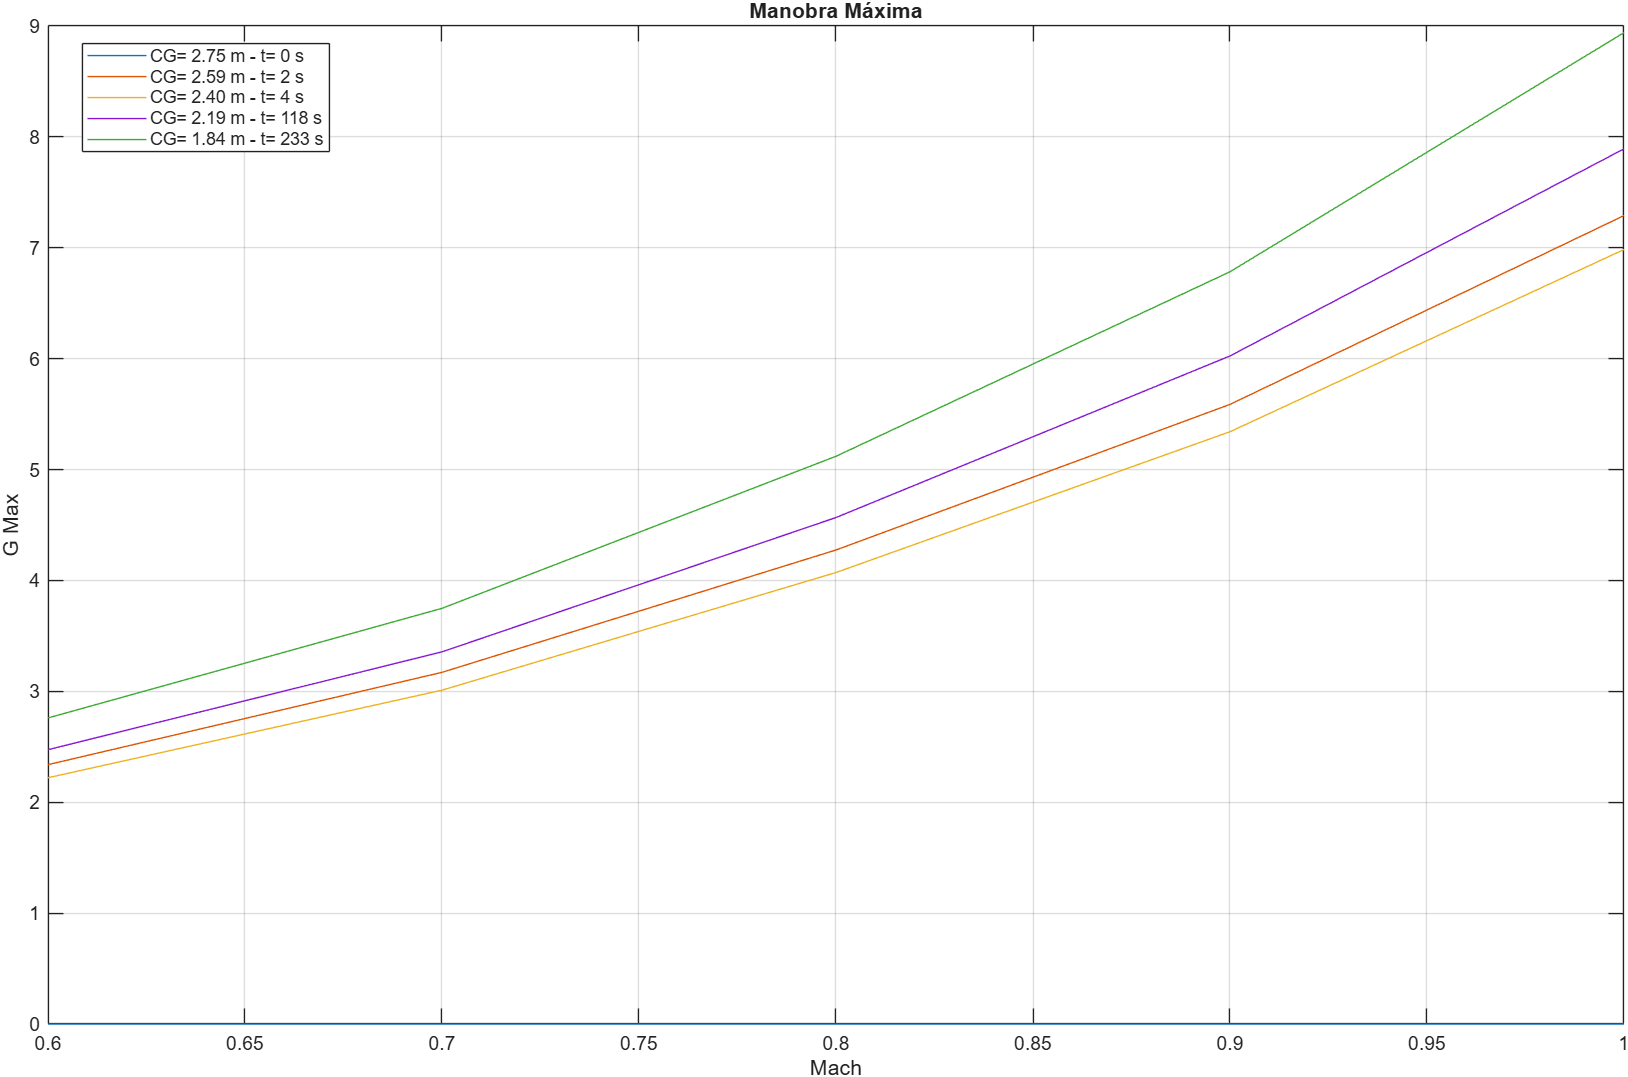
\includegraphics[width=\linewidth]{01_Gmax_manobra_maxima.png}
      \end{center}
      \footnotesize Manobra máxima: todas as fases de CG acham trim;
      terminal a Mach 0{,}9 $\approx 5{,}6\gee$ ($\geq 5\gee$ \chk).
  \end{columns}
\end{frame}

% ================================================================ 4
\section{Aerodinâmica}
\begin{frame}{Aerodinâmica --- DATCOM}
  \begin{center}
    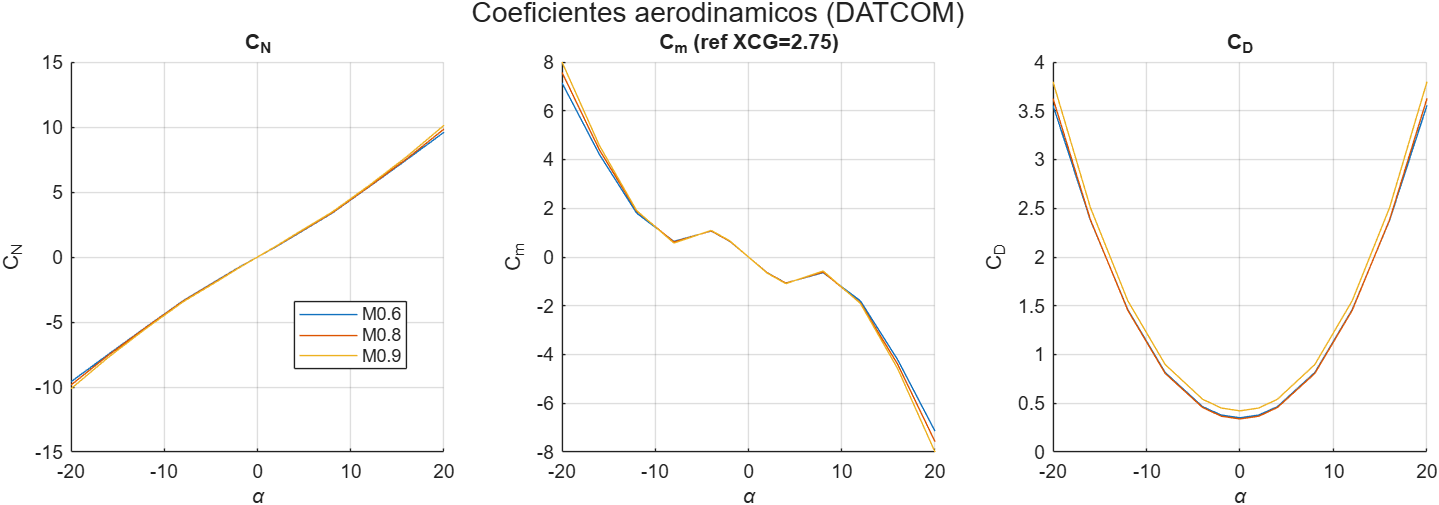
\includegraphics[width=0.92\linewidth]{02_coef_aerodinamicos.png}
  \end{center}
  \footnotesize
  $C_N$ linear (sustentação), $C_m$ com inclinação negativa
  (estaticamente \textbf{estável}), $C_D$ parabólico. Tabelas 3D em
  $(\delta,\text{Mach},\alpha)$ consumidas pela dinâmica 6DOF; derivadas de
  estabilidade por diferenças finitas alimentam as funções de transferência.
\end{frame}

% ================================================================ 5
\section{Dinâmica 6DOF}
\begin{frame}{Dinâmica 6DOF --- por que precisamos do autopiloto}
  \begin{center}
    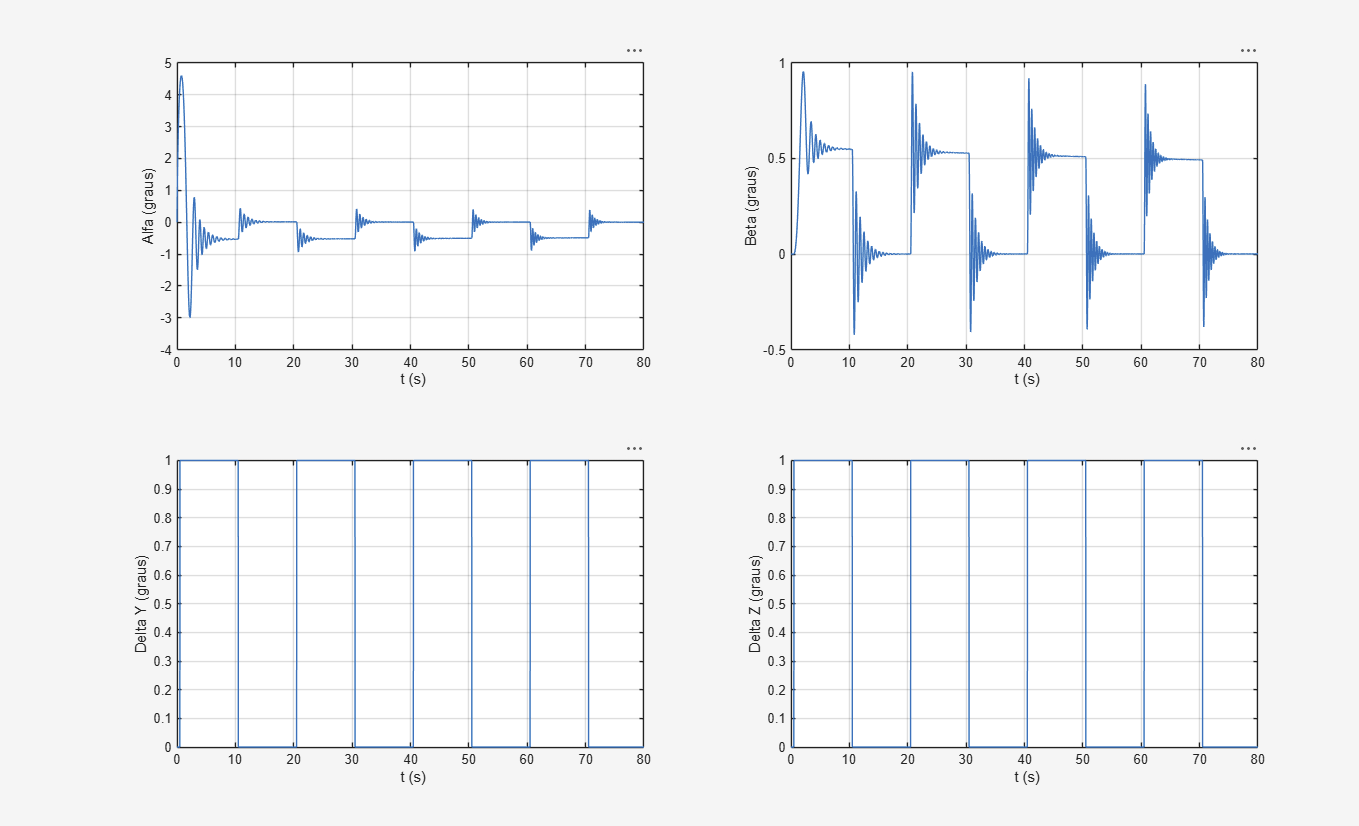
\includegraphics[width=0.82\linewidth]{alphaxdelta.png}
  \end{center}
  \footnotesize
  Resposta \textbf{livre} da célula (malha aberta) a um trem de degraus de
  leme: $\alpha$ e $\beta$ \alert{oscilam e amortecem devagar}
  (curto-período pouco amortecido, $\xi\approx0{,}08$), com a frequência
  subindo conforme o míssil acelera. Daí a necessidade do autopiloto.
\end{frame}

% ================================================================ 6
\section{Autopiloto}
\begin{frame}{Autopiloto --- arquitetura (root locus)}
  \begin{center}
    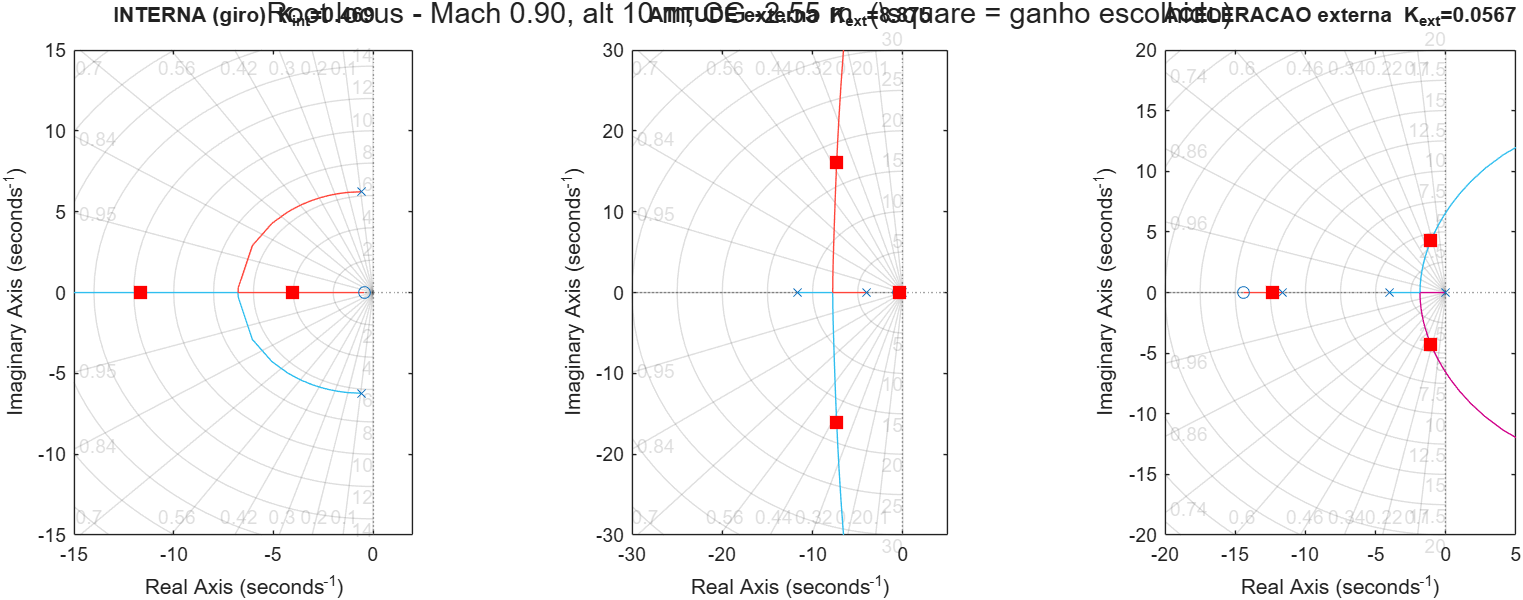
\includegraphics[width=\linewidth]{05_rootlocus.png}
  \end{center}
  \footnotesize
  Três laços projetados por root locus:
  \textbf{interno de girômetro} (amortece o curto-período, $\xi: 0{,}08\to1$),
  \textbf{externo de atitude} ($\zeta\approx0{,}5$) e
  \textbf{externo de aceleração} (limitado pelo zero de fase não-mínima).
  Ganhos escalonados por (CG, altitude, Mach).
\end{frame}

\begin{frame}{Autopiloto --- ganhos e resposta ao degrau}
  \begin{columns}[c]
    \column{0.5\textwidth}
      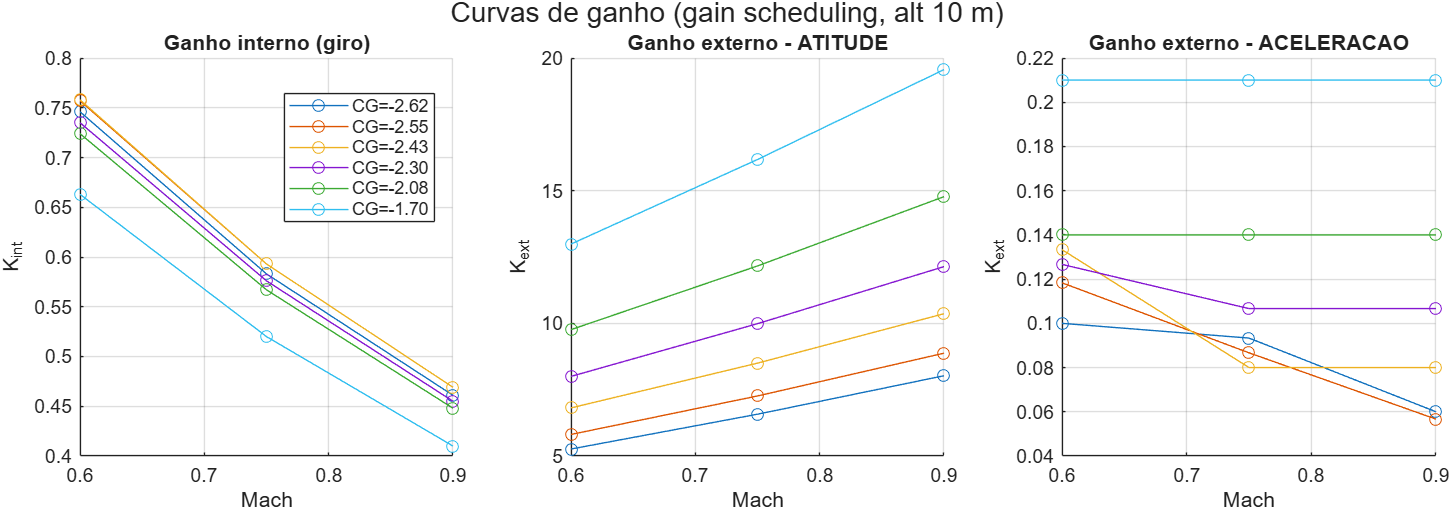
\includegraphics[width=\linewidth]{03_ganhos_autopiloto.png}\\
      \footnotesize\centering Gain scheduling (ganho $\times$ Mach, por CG)
    \column{0.5\textwidth}
      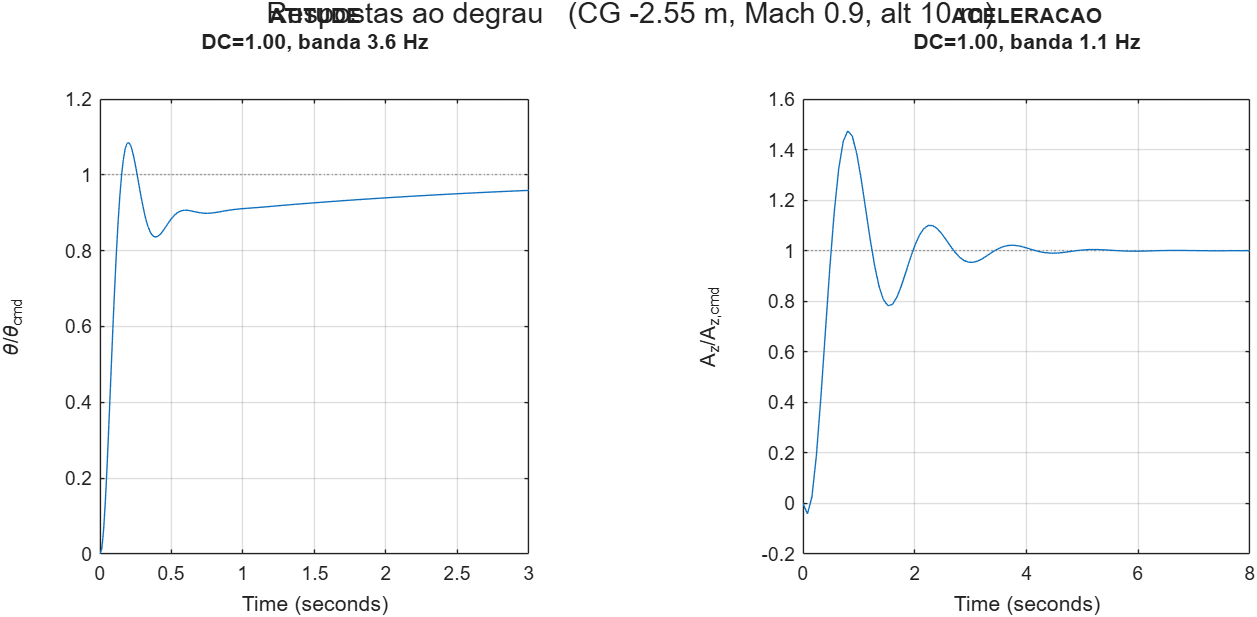
\includegraphics[width=\linewidth]{04_degrau_autopiloto.png}\\
      \footnotesize\centering Degrau: atitude e aceleração, DC${}=1{,}00$,
      banda $2{,}6$--$3{,}6$ Hz / $0{,}7$--$1{,}3$ Hz ($\geq 0{,}5$ Hz \chk)
  \end{columns}
\end{frame}

\begin{frame}{Autopiloto --- segue o comando}
  \begin{columns}[c]
    \column{0.56\textwidth}
      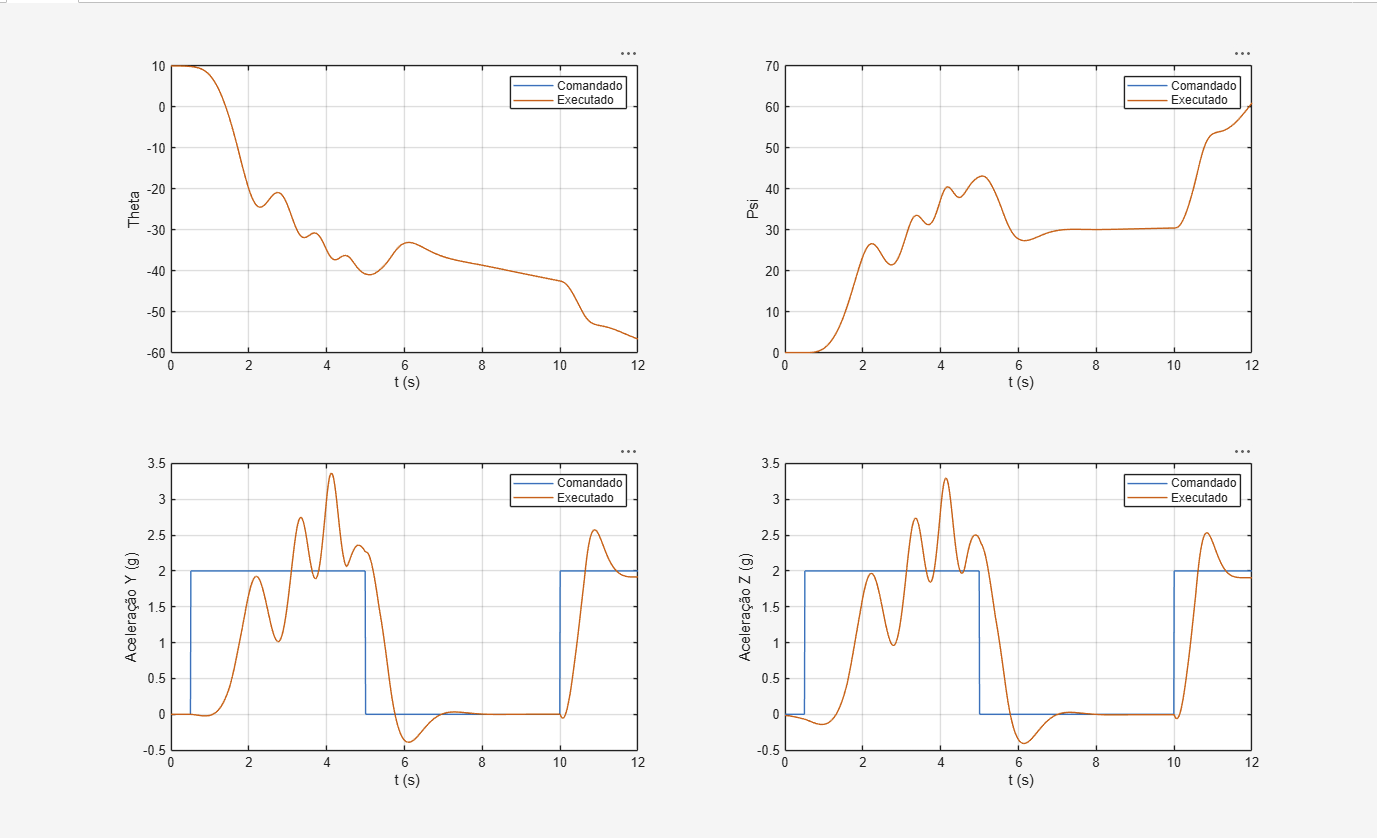
\includegraphics[width=\linewidth]{autoPiloto.png}\\
      \footnotesize\centering 6DOF completo: comandado $\times$ executado
      ($\theta$, $\psi$, $A_y$, $A_z$) --- praticamente coincidem
    \column{0.44\textwidth}
      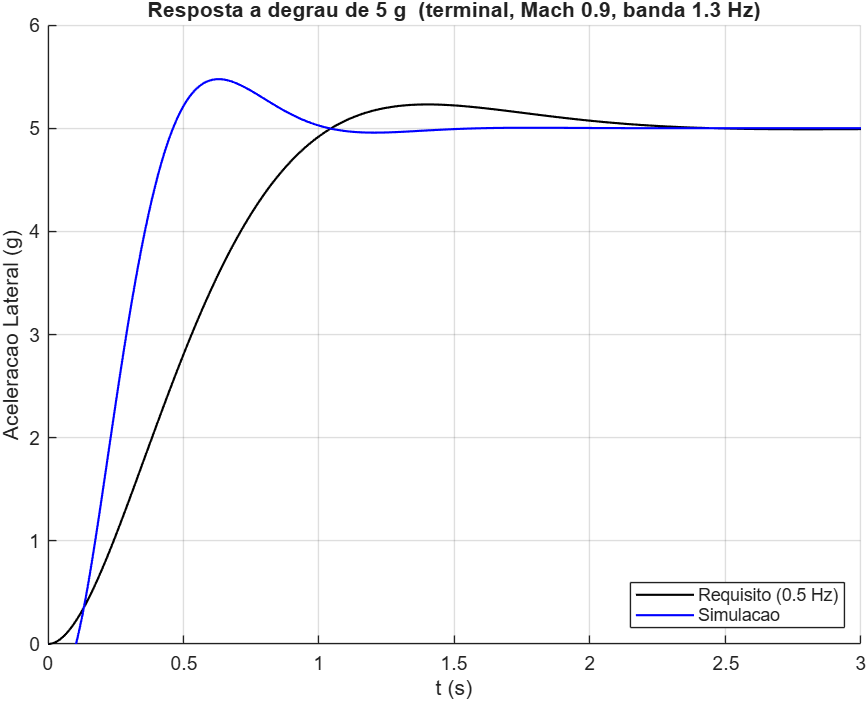
\includegraphics[width=\linewidth]{08_degrau_5g.png}\\
      \footnotesize\centering Degrau de $5\gee$: simulação mais rápida que o
      requisito de banda \chk
  \end{columns}
\end{frame}

% ================================================================ 7
\section{Guiamento}
\begin{frame}{Controle de altitude e guiamento}
  \begin{columns}[T]
    \column{0.5\textwidth}
      \textbf{Sea-skimming}
      \[ \theta_{ref} = \mathrm{sat}_{\pm}\big[K_{Alt}\,(h_{ref}-h)\big] \]
      $K_{Alt}=1^\circ/\text{m}$, estabiliza em $\sim 26$ m.
      \vspace{1em}

      \textbf{Guiamento terminal}
      \[ a_{cmd}\approx N\,V\,\dot\sigma_{LOS}, \quad N=K_{Prop}=3{,}5 \]
      Navegação proporcional + compensação de gravidade; espoleta de
      proximidade $R_{esp}=20$ m.
    \column{0.5\textwidth}
      \begin{block}{Modos de voo}
        \begin{itemize}\small
          \item \textbf{Cruzeiro}: controle de altitude $\rightarrow$
                autopiloto de \textbf{atitude}.
          \item \textbf{Terminal}: autodiretor + nav. proporcional
                $\rightarrow$ autopiloto de \textbf{aceleração}.
        \end{itemize}
      \end{block}
      Autodiretor ideal: ângulos/taxas de LOS via \texttt{atan2}, limitado
      pelo campo de visada ($\pm 40^\circ$).
  \end{columns}
\end{frame}

% ================================================================ 8
\section{Resultados}
\begin{frame}{Resultado --- BINGO}
  \begin{center}
    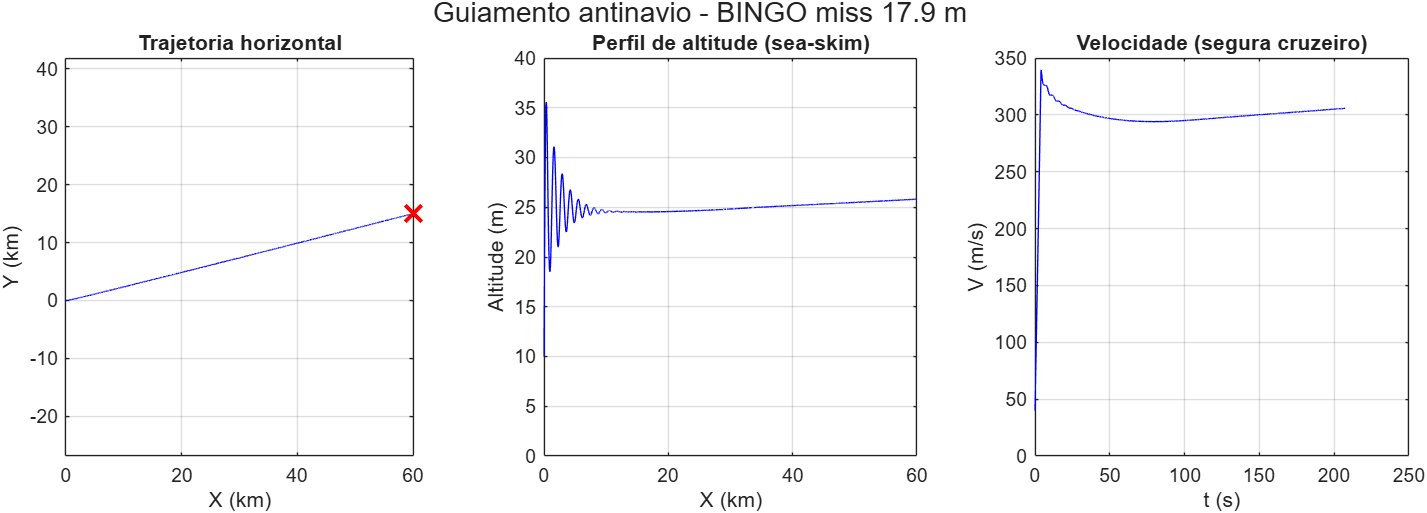
\includegraphics[width=\linewidth]{06_guiamento_trajetoria.png}
  \end{center}
  \footnotesize\centering
  Voo homing a 60 km: \alert{\textbf{miss 17{,}9 m}} ($<$ espoleta 20 m),
  Mach 0{,}90 mantido, sea-skim $\sim 26$ m, $\sim 207$ s.
\end{frame}

\begin{frame}{Resultado --- séries temporais}
  \begin{center}
    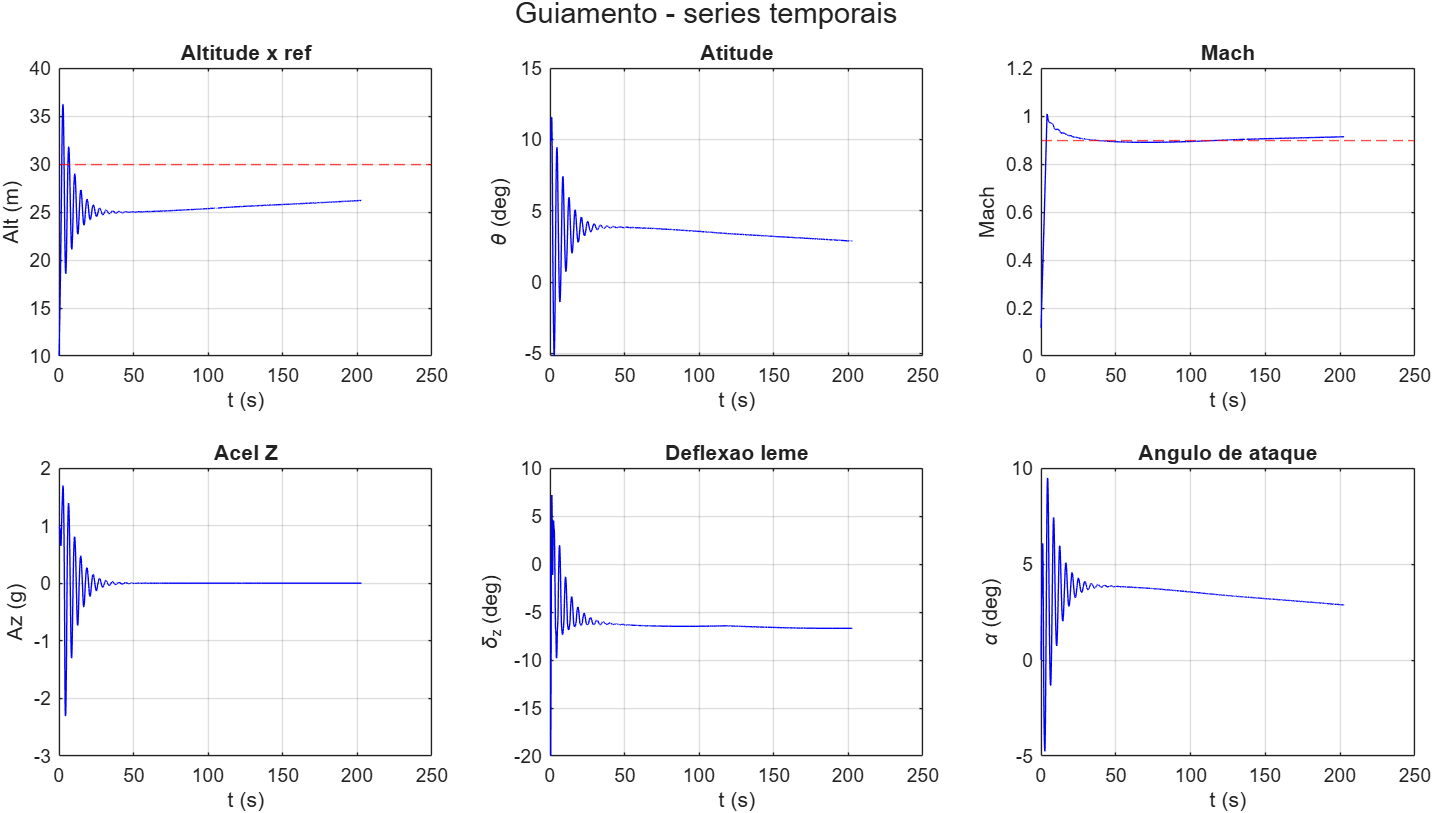
\includegraphics[width=\linewidth]{07_guiamento_series.png}
  \end{center}
  \footnotesize\centering
  Altitude, atitude, Mach, aceleração, leme e $\alpha$. Transiente de boost
  em $0$--$40$ s (baixo Mach), depois cruzeiro liso até o impacto.
\end{frame}

\begin{frame}{Envelope de engajamento}
  \begin{columns}[c]
    \column{0.62\textwidth}
      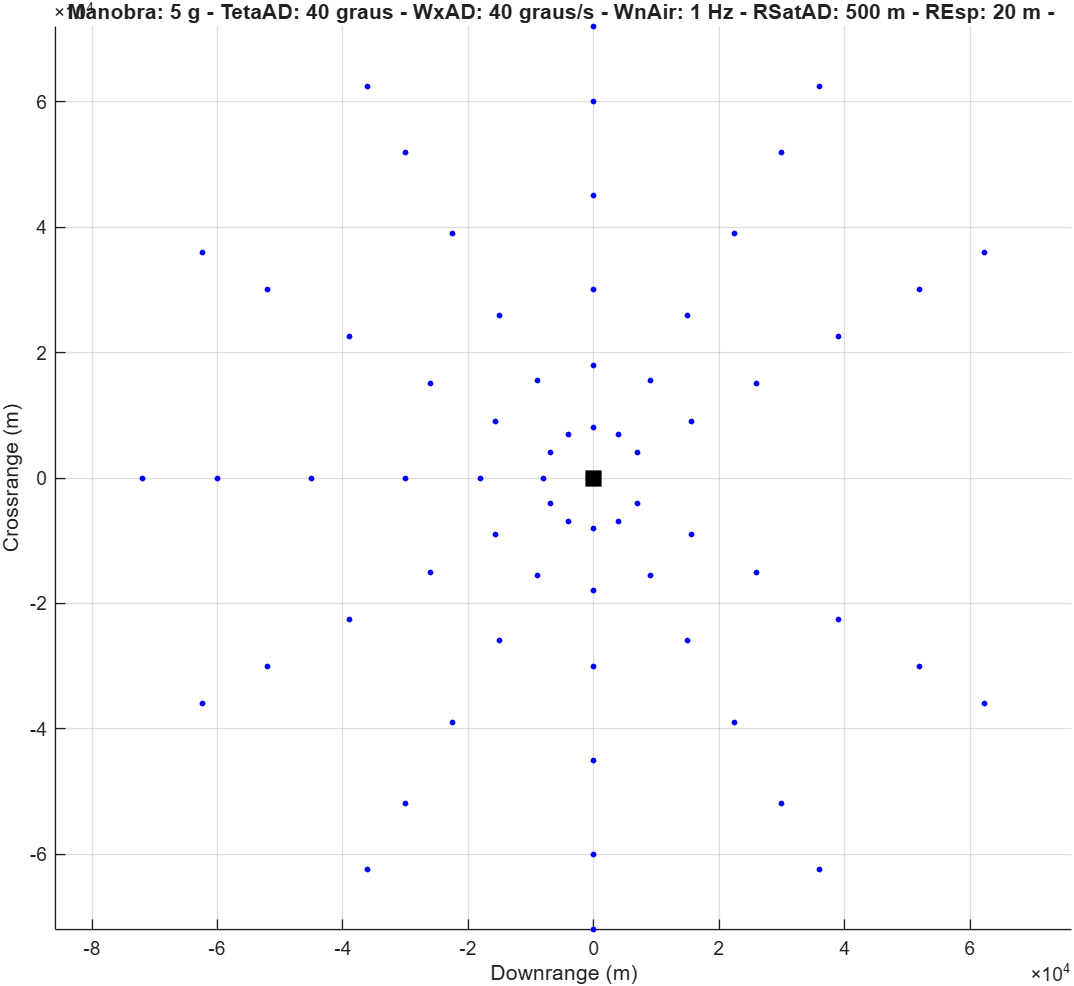
\includegraphics[width=\linewidth]{09_envelope_antinavio.png}
    \column{0.38\textwidth}
      \footnotesize
      Cada ponto azul é um lançamento que biga (estilo da Fig.~10.105 da
      apostila).
      \begin{itemize}
        \item Quase \textbf{omnidirecional} (lançado apontado ao alvo).
        \item Alcance máximo $\sim 72$--$76$ km --- \textbf{excede os 70 km}.
        \item Limitado pela queima do sustainer ($\sim 232$ s).
      \end{itemize}
  \end{columns}
\end{frame}

% ================================================================ 9
\section{Conclusões}
\begin{frame}{Requisitos atendidos}
  \centering
  \begin{tabular}{@{}lll@{}}
    \toprule
    \textbf{Critério} & \textbf{Exigido} & \textbf{Obtido} \\
    \midrule
    Bingo                 & miss $<$ 20 m        & \textbf{17{,}9 m} \ \chk \\
    Manobra lateral       & $\geq 5\gee$         & $\sim 5{,}6\gee$ terminal \ \chk \\
    Banda passante        & $\geq 0{,}5$ Hz      & $2{,}6$--$3{,}6$ / $0{,}7$--$1{,}3$ Hz \ \chk \\
    Cruzeiro              & Mach 0{,}9           & mantido \ \chk \\
    Manobra máx.\ (Gmax)  & trim em $\pm 20^\circ$ & todas as fases \ \chk \\
    Alcance (envelope)    & 70 km                & $\sim 72$--$76$ km \ \chk \\
    \bottomrule
  \end{tabular}
  \vfill
  \footnotesize Sustainer dimensionado para o arrasto de trim; CG à frente
  para fechar o Gmax; autopiloto por root locus com gain scheduling;
  guiamento por navegação proporcional com voo rasante.
\end{frame}

\begin{frame}[plain]
  \begin{center}
    {\Large \textbf{Obrigado!}}\\[1em]
    {\normalsize Míssil Antinavio MANSUP --- PRJ-75 / ITA}\\[0.5em]
    {\footnotesize Perguntas?}
  \end{center}
\end{frame}

\end{document}
